% Volumetric energy U(J) and Kirchhoff pressure p(J) = J U'(J) of the two compressible Neo-Hookean
% models, both normalized by the bulk modulus K.
%   Dissertation (Borden et al.):  U = (K/2)[(J^2-1)/2 - ln J],      p = (K/2)(J^2 - 1)
%   Modified (CNHJay):             U = (K/4)[(J-1)^2 + (1/J-1)^2],  p = (K/2)(J - 1/J)(J + 1/J - 1)
\pgfplotsset{
    cnhaxis/.style={
            width=0.9\linewidth,
            height=0.7\linewidth,
            xmin=0.25, xmax=2.5,
            xlabel={$J$},
            grid=major,
            legend cell align=left,
            legend style={font=\scriptsize},
        },
    cnhborden/.style={blue, line width=1.2pt, domain=0.25:2.5, samples=200},
    cnhjay/.style={red, line width=1.2pt, dashed, domain=0.25:2.5, samples=200},
}
\begin{figure}[htbp]
    \centering
    \begin{subfigure}[t]{0.48\textwidth}
        \centering
        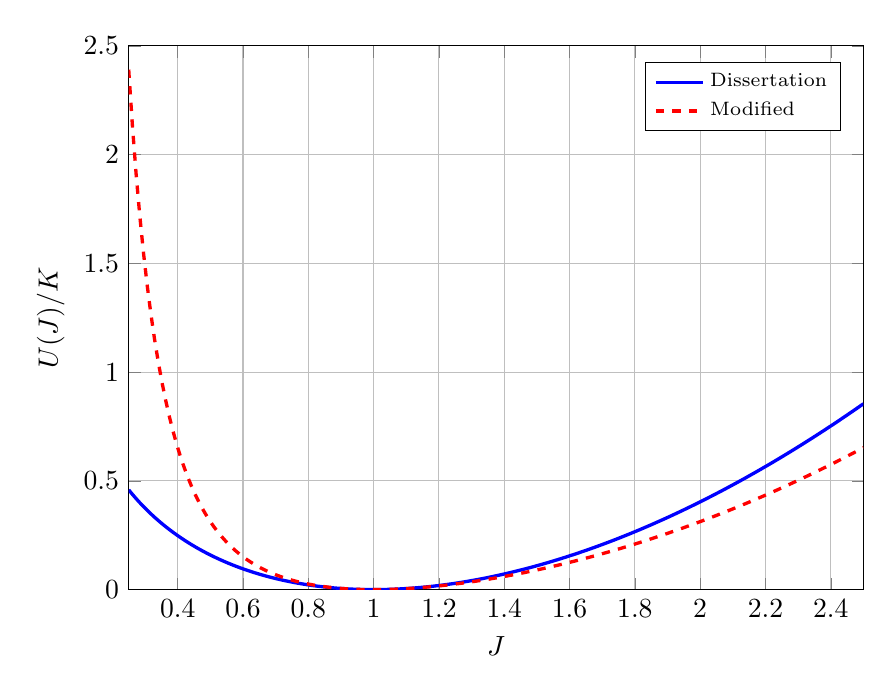
\begin{tikzpicture}
            \begin{axis}[cnhaxis, ymin=0, ymax=2.5, ylabel={$U(J)/K$}, legend pos=north east]
                \addplot[cnhborden] {0.5*(0.5*(x^2-1) - ln(x))};
                \addlegendentry{Dissertation}
                \addplot[cnhjay] {0.25*((x-1)^2 + (1/x-1)^2)};
                \addlegendentry{Modified}
            \end{axis}
        \end{tikzpicture}
        \caption{Volumetric energy}\label{fig:cnh_energy}
    \end{subfigure}
    \hfill
    \begin{subfigure}[t]{0.48\textwidth}
        \centering
        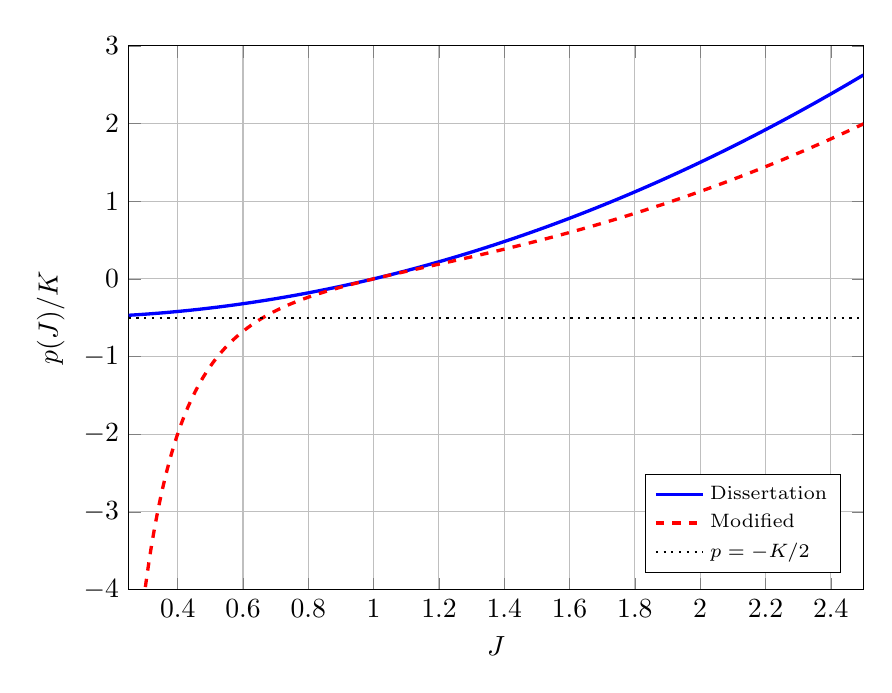
\begin{tikzpicture}
            \begin{axis}[cnhaxis, ymin=-4, ymax=3, ylabel={$p(J)/K$}, legend pos=south east, restrict y to domain=-10:10]
                \addplot[cnhborden] {0.5*(x^2-1)};
                \addlegendentry{Dissertation}
                \addplot[cnhjay] {0.5*(x-1/x)*(x+1/x-1)};
                \addlegendentry{Modified}
                \addplot[black, dotted, line width=0.8pt, domain=0.25:2.5] {-0.5};
                \addlegendentry{$p=-K/2$}
            \end{axis}
        \end{tikzpicture}
        \caption{Volumetric Kirchhoff pressure}\label{fig:cnh_pressure}
    \end{subfigure}
    \caption{Volumetric response of the dissertation's compressible Neo-Hookean model (Eq.~\eqref{eq:cnh_vol_borden}) and the modified model (Eq.~\eqref{eq:cnh_vol_jay}), normalized by the bulk modulus. Both have the same small-strain bulk modulus at $J=1$. As $J\to0$ the dissertation's pressure tends to the finite limit $-K/2$, whereas the modified pressure diverges.}\label{fig:cnh_potentials}
\end{figure}
